\documentclass[12pt]{uthesis-v12}  %---> DO NOT ALTER THIS COMMAND

\usepackage{hyperref}
\usepackage{epigraph}

\usepackage[dvips]{graphicx}
\graphicspath{{images/}}
\DeclareGraphicsExtensions{.eps}


\begin{document} %---> %---> %---> %---> DO NOT ALTER THIS COMMAND

%--------+----------------------------------------------------------+
%        |  \title{}                                    (REQUIRED)  |
%        |  \author{}                                   (REQUIRED)  |
%        |                                                          |
%        |  See section 3.1 of "Read_Me_First_(v12).pdf"            |
%        |                                                          |
%        |  Also see section 2.2 of above "Read Me" file for the    |
%        |  proper use of the invisible tilde ("~") character when  |
%        |  entering a middle initial in the \author command.       |
%        +----------------------------------------------------------+

\title{combox}

\author{Siddharth Ravikumar}

%--------+----------------------------------------------------------+
%        |  \copyrightpage{}                            (REQUIRED)  |
%        |                                                          |
%        |  See section 3.2 of "Read_Me_First_(v12).pdf"            |
%        |                                                          |
%        |  1) You must enter either "yes" or "no" in this          |
%        |      command.  Inputting "yes" produces a copyright      |
%        |      notification page as the second page and inputting  |
%        |      "no" produces a blank second page.                  |
%        |  2) Input to this command is case sensitive.             |
%        |  3) Default: the "yes" option.                           |
%        +----------------------------------------------------------+

\copyrightpage{yes}

%--------+----------------------------------------------------------+
%        |  \mydocument{}                               (REQUIRED)  |
%        |                                                          |
%        |  See section 3.3 of "Read_Me_First_(v12).pdf"            |
%        |                                                          |
%        |  1) Input to this command is limited to the following    |
%        |     three options: a) Dissertation                       |
%        |                    b) Thesis                             |
%        |                    c) Project                            |
%        |  2) Input to this command is case-sensitive.             |
%        +----------------------------------------------------------+

\mydocument{Project}

%--------+----------------------------------------------------------+
%        |  \degree{}{}                                 (REQUIRED)  |
%        |                                                          |
%        |  See section 3.4 of "Read_Me_First_(v12).pdf"            |
%        |                                                          |
%        |  You need to provide two distinct inputs into this       |
%        |  command:                                                |
%        |     1) In the first set of braces you need to specify    |
%        |        the *exact* degree you will receive. Some         |
%        |        examples are: -) Masters of Arts                  |
%        |                      -) Masters of Science               |
%        |                      -) Doctor of Philosophy             |
%        |     2) In the second set of braces you need to state the |
%        |        *specific* discipline or area for that degree     |
%        |        (e.g., Economics, Education, Engineering, etc.).  |
%        |  Students should consult their advisor if they have any  |
%        |  questions about this information.                       |
%        +----------------------------------------------------------+

\degree{Masters of Science}{Computer Science}

%--------+----------------------------------------------------------+
%        |  \conferraldate{}{}                          (REQUIRED)  |
%        |                                                          |
%        |  See section 3.5 of "Read_Me_First_(v12).pdf"            |
%        |                                                          |
%        |  In the two set of braces enter the month and then the   |
%        |  year your degree will be *conferred* by the university. |
%        +----------------------------------------------------------+

\conferraldate{May}{2016}

%--------+----------------------------------------------------------+
%        |  \advisor{}                                  (REQUIRED)  |
%        |                                                          |
%        |  See section 3.6.2 of "Read_Me_First_(v12).pdf"          |
%        |                                                          |
%        |  1) Also see section 2.2 of "Read_Me_First_(v12).pdf"    |
%        |     for the proper use of the invisible tilde ("~")      |
%        |     character when entering a middle initial or the      |
%        |     abbreviation of an academic title (e.g., Dr.) in     |
%        |     the \advisor{} command.                              |
%        |  2) Also see section 3.6.1. for consistent presentation  |
%        |     of title page signature lines.                       |
%        +----------------------------------------------------------+

\advisor{Dr.~Robert C. Green II}

%--------+----------------------------------------------------------+
%        |  Committee Member Signature Commands         (OPTIONAL)  |
%        |                                                          |
%        |  See section 3.6.3 of "Read_Me_First_(v12).pdf"          |
%        |                                                          |
%        |  1) Use the commands below to provide signature lines    |
%        |     for your "other" committee members;                  |
%        |        --> you must list your other committee members    |
%        |            in alphabetic order by last name              |
%        |        --> to do this, use the commands below in the     |
%        |            order presented below.                        |
%        |  2) You can choose to include none, some, or all of the  |
%        |     "XXXmember" commands below --- based on the number   |
%        |     committee members you have; simply delete (or        |
%        |     comment-out) any of the commands below that are not  |
%        |     needed.                                              |
%        |  3) Do not include the name of your committee chair or   |
%        |     the Graduate Dean in the commands listed below.      |
%        |     Their signature lines are generated by the           |
%        |     \advisor{} and \graduatedean{}{} commands.           |
%        |  4) You cannot use any of the commands below more than   |
%        |     once. (For details on this issue, see section 3.6.3  |
%        |     of "Read_Me_First_(v12).pdf".)                       |
%        |  5) Also see section 2.2 of "Read_Me_First_(v12).pdf"    |
%        |     for the proper use of the invisible tilde ("~")      |
%        |     character when entering a middle initial or the      |
%        |     abbreviation of an academic title (e.g., Dr.) in     |
%        |     the commands below.                                  |
%        |  6) See section 3.6.1. for consistent presentation of    |
%        |     title page signature lines.                          |
%        |                                                          |
%        |  I know I shouldn't have to say this, but enough         |
%        |  students over the years have made the same mistake      |
%        |  that I'm forced to state:                               |
%        |                                                          |
%        |      THE NAMES USED IN THE FOLLOWING COMMANDS ARE        |
%        |      SILLY NAMES I'VE USED AS EXAMPLES ONLY.  THEY       |
%        |      ARE NOT THE ACTUAL NAMES OF YOUR COMMITTEE          |
%        |      MEMBERS.  REPLACE THE SILLY NAMES BELOW WITH        |
%        |      THE NAMES OF YOUR ACTUAL COMMITTEE MEMBERS.         |
%        |                                                          |
%        +----------------------------------------------------------+

  \secondmember{Dr.~XX}
   \thirdmember{Dr.~XX}

%--------+----------------------------------------------------------+
%        |  \graduatedean{}{}                           (REQUIRED)  |
%        |                                                          |
%        |  See section 3.6.4 of "Read_Me_First_(v12).pdf"          |
%        |                                                          |
%        |  1) THE NAME AND TITLE PROVIDED BELOW ARE THOSE OF THE   |
%        |     ACTUAL GRADUATE DEAN AT THE TIME THIS DOCUMENT WAS   |
%        |     CONSTRUCTED (January 2012). Contact the Graduate     |
%        |     College to determine whether this information is     |
%        |     correct at the time you submit your document.        |
%        |  2) Section 2.2 of "Read_Me_First_(v12).pdf" describes   |
%        |     the proper use of the invisible tilde ("~")          |
%        |     character when entering a middle initial or the      |
%        |     abbreviation of an academic title (e.g., Dr.) in     |
%        |     the \graduatedean{} command.                         |
%        |  3) See section 3.6.1. for consistent presentation of    |
%        |     title page signature lines.                          |
%        +----------------------------------------------------------+

\graduatedean{Dr.~Michael Ogawa}{Dean}

%--------+----------------------------------------------------------+
%        |  \maketitle                                  (REQUIRED)  |
%        |                                                          |
%        |  See section 3.7 of "Read_Me_First_(v12).pdf"            |
%        |                                                          |
%        |  This is a required LaTeX command; to be brief, bad      |
%        |  things will happen if this command is not included      |
%        |  in your document at this particular location.           |
%        +----------------------------------------------------------+

\maketitle  %---->  ----->  ---->  ---->   DO NOT ALTER THIS COMMAND

%--------+----------------------------------------------------------+
%        |  Abstract Page Environment                   (REQUIRED)  |
%        |                                                          |
%        |  See section 3.8 of "Read_Me_First_(v12).pdf"            |
%        +----------------------------------------------------------+

\begin{abstractpage}
  File storage providers on the Internet have made it non-trivial for
  individuals to store personal files on the file storage provider's
  computers. After Mr. Snowden disclosed information about the
  National Security Agency' (NSA) surveillance programs that allowed
  the NSA to access information stored on file storage provider'
  computers, online file storage became a non-solution for storing
  personal files for everyone who detested the possibility of somebody
  else being able to access their personal files. In the past, there
  have been separate efforts to come with a solution to allow
  individuals to use storage space provided by file storage providers
  in a way that it made it impossible for file storage providers and
  to access the files. combox is one such effort. It allows an
  individual to store personal files in the ``combox directory'' on
  all her computers (running GNU/Linux or OS X) and the combox program
  takes the files, splits and encrypts them and spreads them across
  file storage providers' directories. Therefore, when an individual
  uses storage space provided by file storage providers through
  combox, each file storage provider gets only a part of the file in
  an encrypted form.
\end{abstractpage}

%--------+----------------------------------------------------------+
%        |  Dedication Page Environment                 (OPTIONAL)  |
%        |                                                          |
%        |  See section 3.9 of "Read_Me_First_(v12).pdf"            |
%        |                                                          |
%        |  If both a dedication page and an acknowledgements page  |
%        |  are included in the document, the dedication page must  |
%        |  proceed the acknowledgements page.                      |
%        +----------------------------------------------------------+

\begin{dedication}
  \noindent Dedicated to the
  \verb+$EDITOR+ I use to literally write everything.
\end{dedication}

%--------+----------------------------------------------------------+
%        |  Acknowledgments Page Environment            (OPTIONAL)  |
%        |                                                          |
%        |  See section 3.10 of "Read_Me_First_(v12).pdf"           |
%        |                                                          |
%        |  If both a dedication page and an acknowledgements page  |
%        |  are included in the document, the dedication page must  |
%        |  proceed the acknowledgements page.                      |
%        +----------------------------------------------------------+

\begin{acknowledgments}
  \noindent Dr.~Robert C. Green II who gave me an opportunity to work
  on combox.
\end{acknowledgments}

%--------+----------------------------------------------------------+
%        |  \tableofcontents                            (REQUIRED)  |
%        |  \listoftables                            (CONDITIONAL)  |
%        |  \listoffigures                           (CONDITIONAL)  |
%        |                                                          |
%        |  See sections 3.11 & 3.12 of "Read_Me_First_(v12).pdf"   |
%        |                                                          |
%        |  1) You must include the \tableofcontents command in     |
%        |     your document: the UT Manual requires every          |
%        |     dissertation/thesis to have a detailed table of      |
%        |     contents.                                            |
%        |  2) Including the \listoftables and \listoffigures       |
%        |     commands is "conditional."  See sections 3.12 of     |
%        |     "Read_Me_First_(v12).pdf" for additional details.    |
%        +----------------------------------------------------------+

\tableofcontents  %----->  ----->  ---->  DO NOT ALTER THIS COMMAND
\listoftables \listoffigures

%--------+----------------------------------------------------------+
%        |  \captionformat{}                            (REQUIRED)  |
%        |                                                          |
%        |  See section 3.12.2 of "Read_Me_First_(v12).pdf"         |
%        |                                                          |
%        |  1) You are required to choose between the "hang" or     |
%        |     "align" option for this command.                     |
%        |  2) Input to this command is case sensitive.             |
%        |  3) Default: ``hang'' option.                            |
%        +----------------------------------------------------------+

\captionformat{hang}

%--------+----------------------------------------------------------+
%        |  List of Abbreviations Environment           (OPTIONAL)  |
%        |                                                          |
%        |  See section 3.13 of "Read_Me_First_(v12).pdf"           |
%        |                                                          |
%        |  1) This is an optional section; consult your advisor    |
%        |     to determine whether you need/want to include this   |
%        |     section in your document.                            |
%        |  2) If you do not want a List of Abbreviations simply    |
%        |     delete the material below (and these instructions).  |
%        |  3) If you do want a List of Abbreviations simply        |
%        |     replace the silly material below with the            |
%        |     information relevant to your document.               |
%        |     a. Within the "listofabbreviations" environment      |
%        |        below you must use a separate \abbreviation{}{}   |
%        |        command for each entry in your List of            |
%        |        Abbreviations.                                    |
%        |     b. As the examples below demonstrate, the            |
%        |        information within the first set of braces is     |
%        |        the abbreviation and the information in the       |
%        |        second set of braces is the definition of that    |
%        |        abbreviation.                                     |
%        +----------------------------------------------------------+

\begin{listofabbreviations}

    \abbreviation{YAML}{YAML Ain't Markup Language}
    \abbreviation{CLI}{Command Line Interface}
    \abbreviation{GUI}{Graphical User Interface}
\end{listofabbreviations}


%--------+----------------------------------------------------------+
%        |  Preface Environment                         (OPTIONAL)  |
%        |                                                          |
%        |  See section 3.15 of "Read_Me_First_(v12).pdf"           |
%        +----------------------------------------------------------+

\begin{preface}
42.
\end{preface}

%XXXXXXXXXXXXXXXXXXXXXXXXXXXXXXXXXXXXXXXXXXXXXXXXXXXXXXXXXXXXXXXXXXXX
%XXXXXXXXXXXXXXXXXXXXXXXXXXXXXXXXXXXXXXXXXXXXXXXXXXXXXXXXXXXXXXXXXXXX
%XXXXXXXXXXXXXXXXXXXXXXXXXXXXXXXXXXXXXXXXXXXXXXXXXXXXXXXXXXXXXXXXXXXX
%XXXXXXXXXXXXXXXXXXXXXXXXXXXXXXXXXXXXXXXXXXXXXXXXXXXXXXXXXXXXXXXXXXXX

%--------+----------------------------------------------------------+
%        |  \makebody                                   (REQUIRED)  |
%        |                                                          |
%        |  See section 3.16 of "Read_Me_First_(v12).pdf"           |
%        |                                                          |
%        |  This is a *required* UThesis command; again, bad        |
%        |  things will happen if this command is not included in   |
%        |  your document at this particular location --- see the   |
%        |  file "Read_Me_First_(v12).pdf" for details.             |
%        +----------------------------------------------------------+

\makebody   %------->  ------->  ------->  DO NOT ALTER THIS COMMAND

%XXXXXXXXXXXXXXXXXXXXXXXXXXXXXXXXXXXXXXXXXXXXXXXXXXXXXXXXXXXXXXXXXXXX
%XXXXXXXXXXXXXXXXXXXXXXXXXXXXXXXXXXXXXXXXXXXXXXXXXXXXXXXXXXXXXXXXXXXX
%XXXXXXXXXXXXXXXXXXXXXXXXXXXXXXXXXXXXXXXXXXXXXXXXXXXXXXXXXXXXXXXXXXXX
%XXXXXXXXXXXXXXXXXXXXXXXXXXXXXXXXXXXXXXXXXXXXXXXXXXXXXXXXXXXXXXXXXXXX

%--------+----------------------------------------------------------+
%        |  \chapter{}                                  (REQUIRED)  |
%        |                                                          |
%        |  See section 3.17 of "Read_Me_First_(v12).pdf"           |
%        |                                                          |
%        |  For guidance on using the commands \chapter{},          |
%        |  \section{}, \subsection{}, \subsubsection{}, etc., see  |
%        |  Leslie Lamport's "LaTeX: A Document Preparation         |
%        |  System." Addison Wesley: Reading Massachusetts, 1985.   |
%        +----------------------------------------------------------+

%% 1
\chapter{Introduction}

%% 2
\chapter{Background}

%% 3
\chapter{Literature Review}

%% 4
\chapter{Structure and Design}

\epigraph{In general, when modeling phenomena in science and
  engineering, we begin with simplified, incomplete models. As we
  examine things in greater detail, these simple models become
  inadequate and must be replaced by more refined
  models.}{\textit{Structure and Interpretation of Computer Programs,
    Section 1.1.5}\cite{sicp}}

\section{Structure of combox}

\begin{figure}[h]
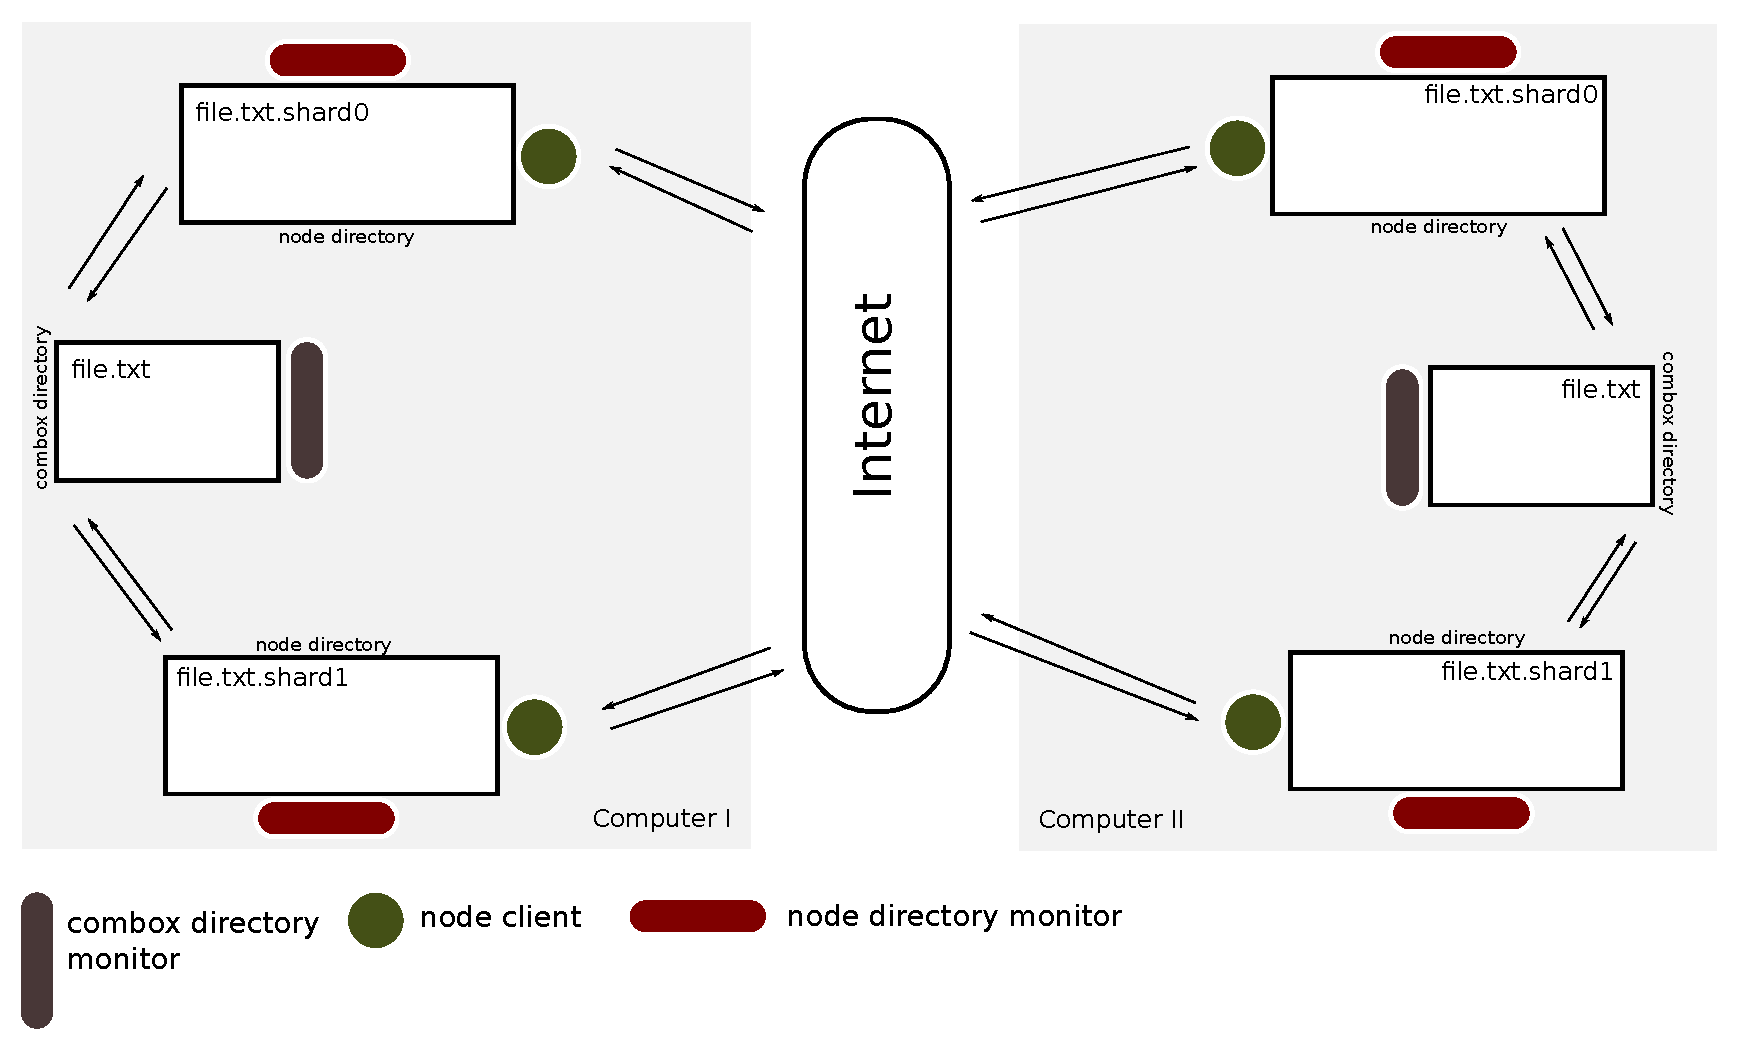
\includegraphics[scale=0.6]{4-combox-structure}
\caption{High level view of combox on two computers.}
\label{fig:4-combox-structure}
\end{figure}

\subsection{combox configuration}

\subsection{combox directory monitor}

\subsection{Node directory monitor}

\subsection{Database structure}

\section{combox modules overview}

combox is spread into modules that have functions and/or classes. As
of \verb+2016-02-04+ combox is considerably a small program:

\begin{verbatim}
$ wc -l combox/*.py
  144 combox/cbox.py
  178 combox/config.py
  241 combox/crypto.py
  891 combox/events.py
  541 combox/file.py
  454 combox/gui.py
    0 combox/__init__.py
   71 combox/log.py
  278 combox/silo.py
   29 combox/_version.py
 2827 total
\end{verbatim}

This section gives an overview of each of the combox modules with
extreme brevity:

\begin{description}
\item[combox.cbox] This module contains \verb+run_cb+ function runs
  combox; it creates an instance \verb+threading.Lock+ for database
  access and a shared \verb+threading.Lock+ for the
  \verb+combox.events.ComboxDirMonitor+ and
  \verb+combox.events.NodeDirMonitor+; it initializes an instance
  \verb+combox.events.ComboxDirMonitor+ that monitors the combox
  directory and an instance of \verb+combox.events.NodeDirMonitor+ for
  each node directory for monitoring the node directories. This
  modules also houses the \verb+main+ function that parses commandline
  arguments, starts combox configuration if needed or loads the combox
  configuration file to start running combox.
\item[combox.config] Accomodates two import functions --
  \verb+config_cb+ and \verb+get_nodedirs+. The \verb+config_cb+ is
  the combox configuration function that allows the user to configure
  combox; this function was designed in a such way that it was
  possible to use for both CLI and GUI methods of configuring
  combox. The \verb+get_nodedirs+ function returns, as a list, the
  paths of the node directories; this function use used in numerous
  places in other combox modules.
\item[combox.crypto] This has functions for encrypting and decrypting
  data; encrypting and decrypting shards (\verb+encrypt_shards+ and
  \verb+decrypt_shards+); a function for splitting a file into shards,
  encrypting those shards and spreading them across node directories
  (\verb+split_and_encrypt+); a function for decrypting the shards
  from the node directories, reconstructing the file from the
  decrypted shards and put the file back to the combox directory
  (\verb+decrypt_and_glue+). Functions \verb+split_and_encrypt+ and
  \verb+decrypt_and_glue+ are the two functions that that are
  extensively used by the \verb+combox.events+ module; all other
  functions in this module are pretty much helper functions are
  \verb+split_and_encrypt+ and \verb+decrypt_and_glue+ functions and
  are not used by other modules.
\item[combox.events] This module took the most time to write and test
  and it is the most complex module in combox at the time of writing
  this report. It contains just two classes -- \verb+ComboxDirMonitor+
  and \verb+NodeDirMonitor+. The \verb+ComboxDirMonitor+ inherits the
  \verb+watchdog.events.LoggingEventHandler+ and is responsible for
  monitoring for changes in the combox directory and doing the right
  thing when change happens in the combox directory. The
  \verb+NodeDirMonitor+ also inherits
  \verb+watchdog.events.LoggingEventHandler+ and similarly responsible
  for monitoring a node directory and doing the right thing when a
  change happens in the node directory; subjectively,
  \verb+NodeDirMonitor+ is slightly more complex than the
  \verb+ComboxDirMonitor+.
\item[combox.file] This is the second largest module in combox. It
  contains utility functions for reading, writing, moving
  files/directiores, hashing files, splitting a file into shards, glue
  shards into a file, manipulating directories inside combox and node
  directories.
\item[combox.gui] Contains the \verb+ComboxConfigDialog+ class; it is
  the graphical interface for configuring combox. The class uses the
  Tkinter library\cite{pylib:tkinter} for spawing graphical
  elements. Other graphical libraries include PyQt\cite{pylib:qt}
  were considered Tkinter was chosen over others because it works on
  all Unix systems and Microsoft's Windows and it is part of the core
  python (version 3).
\item[combox.log] All the messages to \verb+stdout+ and \verb+stderr+
  are sent through the functions \verb+log_i+ and \verb+log_e+
  functions defined in this module.
\item[combox.silo] Contains the \verb+ComboxSilo+ class which is the
  canonical interface for combox for managing information about the
  files in the combox directory. Internally, the \verb+ComboxSilo+
  class uses the pickleDB library\cite{pylib:pickledb}.
\item[combox.\_version] This is \emph{private} module that contains
  variables that contain the value of the present version and release
  of combox. The \verb+get_version+ function in this module returns
  the full version number; this function used by \verb+setup.py+.
\end{description}

\section{Language choice}

Back in October of 2014, I was learning to write in python and when I
had to start working on combox, I chose to write combox in python. In
my first commit to the combox repository, I had say say this about
python:

\begin{verbatim}
commit 2def977472b2e77ee88c9177f2d03f12b0263eb0
Author: rsiddharth <rsiddharth@ninthfloor.org>
Date:   Wed Oct 29 23:24:58 2014 -0400

    Initial commit: File splitter & File gluer done.

    ...

    I like to write python FWIW. But after reading a dialect of Lisp when
    I come back to python, it does not look very beautiful. I guess I'm
    pretty convinced that there is no language that can ape the beauty of
    Lisp.
\end{verbatim}

If I were to write that commit message today (\verb+2016-02-04+), I
would've phrased my reflections about python differently. While I've
not found a language that is as intrinsically beautiful as Lisp, I'm
not sure if it is not quite right to compare Lisp and Python. Python
is a very readable language and it tends to be very accessible to
beginners. Also, it is hard to write unreadable Python code.

\section{DRY}

The core functionality of combox is to split, encrypt file shards,
spread them across node directories (Google Drive and Dropbox) and
decrypt, glue shards and put them back to the combox directory when a
file is created/modified/deleted/moved in another computer. The plan
was to use external libraries to accomplish things fell outside the
realm of what I consider the ``core functionality of combox''; the
main reason behind this decision was to duly be an indolent programmer
and not indulge in trying to solve problems that others have already
solved.

The \verb+watchdog+\cite{pylib:watchdog} library used for file
monitoring; this library is compatible with Unix systems and
Windows. The \verb+pycrypto+ library\cite{pylib:pycrypto} was used for
encrypting data; combox uses AES encryption scheme to encrypt file
shards. The \verb+pickleDB+ library was used to store information
about files in the combox directory; this library is not very clean
but it was what I exactly looking for, if there was no
\verb+pickleDB+, I would've most probably written something similar to
it and made it as part of combox.

Looking back, the decision to use external libraries reduced the
complexity of combox, reduced the time to complete the initial working
version of combox and made it possible to spend more than 3 months
just testing and fixing issues in combox.

\section{Operating system compatibility}\label{4-os-compat}

\section{combox as a python package}

\section{With the benefit of hindsight}


%% 5
\chapter{Testing}

\epigraph{Testing shows the presence, not the absence of
  bugs.}{\textit{Dijkstra}\cite{dijkstra69}}

\section{Unit testing}

The \verb+nose+\cite{pylib:nose} testing framework was used to
write unit tests for the functions and classes part of the
\verb+combox.config+, \verb+combox.crypto+, \verb+combox.events+,
\verb+combox.file+, \verb+combox.silo+ \verb+combox._version+
modules. Unit tests were not written for \verb+combox.cbox+,
\verb+combox.gui+, \verb+combox.combox.log+ modules.

Unit tests for combox become reality by pure serendipity. During the
time, when I started working on combox, I was learning to use the
\verb+nose+ library to unit test python code. Since, \verb+combox+ was
being written in python, I started making it a norm to write unit
tests for functions and classes in combox modules.

As mentioned before, unit tests were not written for some modules
either because it would make no sense to write one (for the
\verb+combox.cbox+ module, for instance, which basically uses
functions and classes defined in other modules to run combox) or it
was not clear how to write unit tests it (the \verb+combox.gui+
contains just the \verb+ComboxConfigDialog+ a graphical front-end
which uses the configuration function defined in the
\verb+combox.config+ module to complete the combox configuration based
on the user input).

It must be noted here that pure Test Driven Development (TDD) was not
observed -- most of the time the function/class was written before the
its corresponding test was written.

\subsection{Benefits}

While writing unit tests definitely increased the time to write a
particular feature, it enabled me to immediately check if a feature
worked as it should for the given use case or given set of inputs.

With the benefit of hindsight, unit tests greatly helped in testing
the compatibility of combox on OSX. Before the \verb+v0.1.0+ release,
combox's node directory monitor always assumed that a file's first
shard (\verb+shard0+) is always available; while this assumption did
not create any problems on GNU/Linux, on OS X, this assumption made
the node directory monitor to behave erratically -- this issue (bug
\#4\cite{combox-issue-tracker} was immediately found when the unit
tests were run for the first time on OS X. Another instance where unit
tests helped was just before the \verb+v0.2.0+ release; major changes,
including the introduction of file locks in the
\verb+ComboxDirMonitor+, were made to the \verb+combox.events+. When
the unit tests were run OS X, two tests failed, revealing a difference
in behavior of watchdog\cite{pylib:watchdog} on GNU/Linux and OS X on
file creation\cite{combox-wd-fix}; without unit tests, there is a high
probability that this bug would never have been found by now.

\subsection{Caveats}

Unit tests are helpful in testing the correctness of a feature for
\verb+N+ number of use cases but it does not necessarily mean the
written feature correctly behaves for use cases that the author of the
feature did not consider or did not think about while writing the
respective feature. As Dijkstra correctly observed:

Unit tests failed to reveal bugs \#4, \#5 \#6 \#7 \#5 \#10
\#11\cite{combox-issue-tracker}; these bugs were found when manually
testing combox.

\section{Manual testing}

The unit tests for the \verb+combox.events+ module test the
correctness of the \verb+ComboxDirMonitor+ and \verb+NodeDirMonitor+
independently; in order to comprehensively test the correctness of
both \verb+ComboxDirMonitor+ and \verb+NodeDirMonitor+, it was
required to manually test combox running on more than one computer. As
you'll see in the following subsections, several bugs were found and
fixed while doing manual testing.

Three different types of setups were used to test combox. The first
kind of setup has two GNU/Linux machines each using combox to sync
files between each other with Dropbox and Google Drive being the
nodes; the second kind of setup has a GNU/Linux machine and a OS X
machine each using combox to sync files between each other with
Dropbox and Google Drive being the nodes; the third kind of setup has
a GNU/Linux machine and OS X machine each using combox to sync files
between each other with Dropbox, Google Drive and a USB stick as
nodes.

\subsection{General setup and notes}

\begin{itemize}
\item On the GNU/Linux machines, the official Dropbox client was used
  to sync the Dropbox node directory to Dropbox'
  servers. \verb+rclone+\cite{program:rclone} was used to sync the
  Google Drive node directory to Google Drive' servers;At the time of
  testing, Google Drive did not have client for GNU/Linux.
\item On OS X, the official Dropbox client was used to sync the
  Dropbox node directory to Dropbox's servers; the official Google
  Drive client was used to sync the Google Drive node directory to
  Google Driver' servers.
\item Since combox is extremely event-driven, combox must be started
  before the Dropbox and Google Drive clients start syncing their
  respective directories (nodes).
\end{itemize}

\subsection{Testing on two GNU/Linux machines}

combox was run to two GNU/Linux machines and a file was alternatively
created/modified/renamed/deleted on an of the GNU/Linux machine and it
was verified if the respective file was also
created/modified/renamed/deleted on the other GNU/Linux machine. One
of the GNU/Linux machine (\verb+lyra)+ was a virtual machine running
Debian GNU/Linux stable (version 8.x); the other GNU/Linux machine
(\verb+grus+) was a physical machine running Debian GNU/Linux
testing. The node directories to scatter the files' shards were the
Dropbox directory and Google Drive directory. The official Dropbox
client was used to automatically sync files from the Dropbox directory
to the Dropbox' server; \verb+rclone+\cite{program:rclone} was used to
sync files from Google Drive directory to Google Drive' server.

\subsubsection{Issues found}\label{ch-5-2gnus-issues}

\begin{itemize}
\item Some editors, especially on POSIX complaint systems, create
  backup version of the file being edited. combox was detecting this
  backup file as a ``new file'' and it split it into shards, encrypted
  the shards and scattered the shards across the node directories. The
  right thing for combox to do was to ignore these backup files and do
  nothing about them. This issue was fixed on
  \verb+2015-09-29+\cite{combox-issue-tracker}. Now the
  \verb+ComboxDirMonitor+, on a ``file created'' or ``file modified''
  event, returns from the \verb+on_created+ or \verb+on_modified+
  callback when it finds that the file is a backup/temporary file.
\item Dropbox client maintains the \verb+.dropbox.cache+ directory
  under the root of the Dropbox directory.

  \begin{itemize}
  \item When a file (shard) was created on another computer, the
    Dropbox client pulls the new file (shard) to this computer into
    \verb+.dropbox.cache+ as a temporary file and then moves the new
    file (shard) to its respective location with the appropriate name.
  \item When a file (shard) was modified on another computer, the
    Dropbox client pulls the modified file (shard) to this computer
    into the \verb+.dropbox.cache+ as a temporary file; moves the old
    version of the file (shard) under the Dropbox directory into the
    \verb+.dropbox.cache+; finally moves the updated copy of the file,
    stored as a temporary file, into the Dropbox directory to its
    respective location with the appropriate name.
  \item When a file (shard) was deleted on another computer, the
    Dropbox client moves the delete file into the
    \verb+.dropbox.cache+ directory on this computer.
  \end{itemize}

  All of the above behavior of the Dropbox client epically broke
  combox. Commits \verb+3d714c5+ to
  \verb+6e1133f+\cite{git:dropbox-fix} fixed combox by making it aware
  of Dropbox's client behavior.
\end{itemize}

\subsubsection{Demo}

Demo of combox being used on two GNU/Linux machines can be viewed at
\url{https://ricketyspace.net/combox/combox-2-gnus.webm}.

\verb+lyra+ (virtual machine) and \verb+grus+ (bare-metal) are the two
GNU/Linux machines being used for the demo.

Description of what happens in the demo follows:

 - (lyra) install combox.

 - (lyra) run combox (test mode).

 - (lyra) create file \verb+walden.pond+ with content ``It must be
 beautiful there''.

 - (lyra) sync Google Drive using \verb+rclone+.

 - (grus) sync Google Drive using \verb+rclone+.

 - (grus) git pull latest copy of combox.

 - (grus) install combox 

 - (grus) run combox (testing mode).

 - (grus) verify that \verb+walden.pond+ was create on this machine.

 - (grus) append 'Peaceful too.' to \verb+walden.pond+.

 - (grus) sync Google Drive using \verb+rclone+.

 - (lyra) sync Google Drive using \verb+rclone+.

 - (lyra) verify that the latest copy of \verb+walden.pond+ is there
 in the combox directory; it should contain 'Peaceful too.' in the
 last line.

 - (lyra) append ``I've a dream'' to \verb+walden.pond+.

 - (lyra) sync Google Drive using \verb+rclone+.

 - (grus) sync Google Drive using \verb+rclone+.

 - (grus) verify that the latest copy of \verb+walden.pond+ is there
 in the combox directory; it should contain ``I've a dream'' in the
 last line.

 - (grus) remove \verb+walden.pond+ from combox directory.

 - (grus) sync Google Drive using \verb+rclone+.

 - (lyra) sync Google Drive using \verb+rclone+.

 - (lyra) verify that \verb+walden.pond+ is removed from the combox
 directory.

 - (grus) open dropbox and Google drive accounts from the web browser.

 - (lyra) create file \verb+manufacturing.consent.+ with content ``Chomsky stuff?''.

 - (lyra) sync Google Drive using \verb+rclone+.

 - (grus) sync Google Drive using \verb+rclone+.

 - (grus) verify that \verb+manufacturing.consent+ was created in the
 combox directory.

 - (grus) verify that the shards of \verb+manufacturing.consent+ were
 created on Dropbox and Google Drive through the web browser.

\subsection{Testing on a GNU/Linux and an OS X machine}

combox was run on a GNU/Linux machine and an OS X machine and a file
was alternatively created/modified/renamed/deleted on one of the
machine and it was verified if the respective file was also
created/modified/renamed/deleted on the other machine. The GNU/Linux
machine was a virtual machine (\verb+lyra+) running Debian GNU/Linux
stable; the OS X machine was on Mavericks (10.9) during the initial
stage of testing, later it was upgraded to Yosemite (10.10). The node
directories to scatter files' shards were the Dropbox directory and
the Google Drive directory. The official Dropbox client was used to
automatically sync files from the Dropbox directory to the Dropbox'
server on both the GNU/Linux machine and the OS X machine; the
official Google Drive client was used to automatically sync files from
the Google Drive directory to Google Drive' server on OS X and
\verb+rclone+\cite{program:rclone} was used to sync files from the
Google Drive directory to Google Drive's server on GNU/Linux.

\subsubsection{Issues found}

\begin{itemize}
\item When a file was modified on another computer, on this computer
  combox assumed that first shard (shard0) will be updated first and
  also counted on the existence of the first shard (shard0). It was
  observed that the order in which the shards were updated were
  unpredictable on this computer and if the first shard (shard0) was
  stored in the Dropbox directory, it will momentarily disappear
  before the most updated shard becomes available in the Dropbox
  directory; this broke combox. This issue was fixed on
  2015-08-25\cite{git:bug-four-fix}. This issue is not got to do with
  the nature of the setup but it is related to the Dropbox's behavior
  elaborated in section \ref{ch-5-2gnus-issues}.
\item The official Google Drive client when it pulls an updated
  version of the file from Google Drive' server, instead directly
  updating the respective file on the computer, it deletes the older
  version of the file and creates the latest version of the file at
  the respective location in the Google Drive directory; this behavior
  of the Google Drive confused and broke combox. This issue was fixed
  2015-09-06 by making combox under the official Google Client's
  behavior\cite{git:bug-googledc-fix}.
\item When a non-empty directory was move/renamed on another computer,
  the old directory was not getting properly deleted on this computer;
  this was happening because the files under the directory being
  renamed were not deleted when it was time for \verb+NodeDirMonitor+
  to \verb+rmdir+ the old directory. This issue again is not specific
  to the nature of the setup but was found while testing combox on
  this setup. This issue was fixed on
  2015-09-12\cite{git:bug-six-fix}.
\item It was found that \verb+combox.file.rm_path+ function failed
  when it was given a non-existent path to remove; this issue was
  fixed on 2015-09-12\cite{git:bug-seven-fix}.
\end{itemize}

\subsubsection{Demo}

Demo of combox being used on a GNU/Linux machine and OS X machine can
be viewed at \url{https://ricketyspace.net/combox/combox-gnu-osx.webm}

\verb+lyra+ is the GNU/Linux (virtual) machine and
\verb+dhcp-129-1-66-1+ is the OS X machine that is being used for the
demo. The OS X machine is accessed through VNC\cite{article:vnc}.

Description of what happens in the demo follows:

  - (\verb+lyra+) create file \verb+cat.stevens+ with content ``peace train''.

  - (\verb+lyra+) sync Google Drive using \verb+rclone+.

  - (\verb+dhcp-129-1-66-1+) verify that file \verb+cat.stevens+ is
  created with content ``peace train''.

  - (\verb+dhcp-129-1-66-1+) append string ``moonshadow'' to file
  \verb+cat.stevens+.

  - (\verb+lyra+) sync Google Drive using \verb+rclone+.

  - (\verb+lyra+) verify that the file \verb+cat.stevens+ was updated
  (modified); last line must have the string ``moonshadow''.

  - (\verb+lyra+) append string ``father and son'' to the file
  \verb+cat.stevens+.

  - (\verb+lyra+) sync Google Drive using \verb+rclone+.

  - (\verb+dhcp-129-1-66-1+) verify that the file \verb+cat.stevens+
  was updated (modified); last line must have the string ``father and
  son''.

  - (\verb+dhcp-129-1-66-1+) rename file \verb+cat.stevens+ to
  \verb+yusuf.islam+

  - (\verb+lyra+) sync Google Drive using \verb+rclone+.

  - (\verb+lyra+) verify that the file \verb+cat.stevens+ was renamed
  to \verb+yusuf.islam+.

\subsection{Testing with a USB stick as a node}

combox was run on a GNU/Linux machine and an OS X machine and a file
was alternatively created/modified/deleted on one of the machine and
it was verified if the repsective file was also
create/modified/deleted on the other machine. The GNU/Linux machine
was a physical machine (\verb+grus+) running Debian GNU/Linux stable;
The OS X machine was on Mavericks (10.9). The node directories to
scatter files' shards were the Dropbox directory, Google Drive
directory and the USB stick (\verb+ZAPHOD+, FAT filesystem). The
official Dropbox client was used to automatically sync files from
Dropbox directory to Dropbox' server on both the GNU/Linux machine and
OS X machine; the official Google Drive client was used to
automatically sync files from the Google Drive directory to Google
Drive' server on OS X and \verb+rclone+\cite{program:rclone} was used
to sync files from the Google Drive directory to Google Drive's server
on GNU/Linux; the same USB stick (\verb+ZAPHOD+) was used on bothe
GNU/Linux and Dropbox to store the third shard (shard2) of a file.

\subsubsection{Caveats}

\begin{itemize}
\item When a removable USB disk is used as a node, combox must be
  turned off before ejecting/unmounting the USB disk; combox does not
  expect a node directory to disappear when it is running, if the USB
  disk is removed when combox is running, then combox goes to a
  undefined state.

\item When a file modified on machine A is synced to machine B, combox
  must be turned on first before turning on Dropbox and Google Drive
  clients and the shard in the USB disk needs to be ``touched'' for
  combox to detect that the file was modified on the remote computer
  and update the file locally on this machine.

\item File rename/move does not work. To make it work, core
  functionality of combox must be re-written.
\end{itemize}

\subsubsection{Demo}

Demo of combox being used with a USB stick as the third node can be
view at \url{https://ricketyspace.net/combox/combox-usb-node-demo.webm}

\verb+grus+ is the GNU/Linux machine and \verb+dhcp-129-1-66-1+ is the
OS X machine that is being used for the demo. \verb+ZAPHOD+ is the
FAT32 USB stick used as the third node.

Description of what happens in the demo follows:

  - (\verb+grus+) start combox.

  - (\verb+grus+) create a file called \verb+simon.and.garfunkel+ with
  content ``the boxer''.

  - (\verb+grus+) sync Google Drive using \verb+rclone+.

  - (\verb+grus+) stop combox.

  - (\verb+grus+) unmount USB stick (\verb+ZAPHOD+) from \verb+grus+.

  - (\verb+dhcp-129-1-66-1+) mount USB stick (\verb+ZAPHOD+) to
  (\verb+dhcp-129-1-66-1+).

  - (\verb+dhcp-129-1-66-1+) start Dropbox client.

  - (\verb+dhcp-129-1-66-1+) start Google Drive client.

  - (\verb+dhcp-129-1-66-1+) start combox.

  - (\verb+dhcp-129-1-66-1+) verify that the file
  \verb+simon.and.garfunkel+ with content ``the boxer'' was created.

  - (\verb+dhcp-129-1-66-1+) append string ``mrs. robinson'' to file
  \verb+simon.and.garfunkel+.

  - (\verb+dhcp-129-1-66-1+) stop combox.

  - (\verb+dhcp-129-1-66-1+) stop Google Drive client.

  - (\verb+dhcp-129-1-66-1+) stop Dropbox client.

  - (\verb+dhcp-129-1-66-1+) unmount the USB stick (\verb+ZAPHOD+)
  from (\verb+dhcp-129-1-66-1+).

  - (\verb+grus+) mount the USB stick (\verb+ZAPHOD+) to
  (\verb+grus+).

  - (\verb+grus+) start combox.

  - (\verb+grus+) start Dropbox client.

  - (\verb+grus+) sync Google Drive using \verb+rclone+.

  - (\verb+grus+) touch \verb+simon.and.garfunkel.shard2+ in the USB
  stick (\verb+ZAPHOD+).

  - (\verb+grus+) verify that the file \verb+simon.and.garfunkel+ is
  updated; the last line must contain the string ``mrs. robinson''.

  - (\verb+grus+) remove the file \verb+simon.and.garfunkel+.

  - (\verb+grus+) sync Google Drive using \verb+rclone+.

  - (\verb+grus+) unmount the USB stick (\verb+ZAPHOD+) from
  (\verb+grus+).

  - (\verb+grus+) stop Dropbox client.

  - (\verb+dhcp-129-1-66-1+) mount the USB stick (\verb+ZAPHOD+) to
  (\verb+dhcp-129-1-66-1+).

  - (\verb+dhcp-129-1-66-1+) start Google Drive client.

  - (\verb+dhcp-129-1-66-1+) start Dropbox client.

  - (\verb+dhcp-129-1-66-1+) start combox.

  - (\verb+dhcp-129-1-66-1+) verify that the file
  \verb+simon.and.garfunkel+ was deleted.


\section{Stress testing}

Large number of files of different sizes were dumped to the combox
directory between an one second interval to see how combox responds to
high load. The file dump size was varied from \verb+424.798190MiB+ (27
files) to \verb+10800.000000MiB+ (180 files); the average time taken
to split a file and the total time to process all files were
calculated for each dump.

Stress testing was first done on \verb+2015-11-08+. In mid November
the \verb+ComboxDirMonitor+ was drastically modified to make it use
the file Lock shared the instances of
\verb+NodeDirMonitor+\cite{git:bug-eleven-fix}; my hunch was that this
change in \verb+ComboxDirMonitor+ directly affected the performance of
combox and therefore the results that were got from stress testing on
\verb+2015-11-08+ would no longer be valid. Stress testing was again
done on \verb+2016-01-16+; the results of this stress test are in
sections \ref{5-st-424} to \ref{5-st-10800}, section \ref{5-st-tu}
gives information about the tools used for stress testing, section
\ref{5-st-o} contains the observations and comparisons between this
stress test and the one done on \verb+2015-11-08+, lastly section
\ref{5-st-if} reveals the issues that were found with combox by virtue
of doing the stress tests.

\subsection{flac dump (27 files - 424.798190MiB)}\label{5-st-424}

\begin{center}
\begin{tabular}{ll}
field & value\\
\hline
delay between a file dump & 1s\\
start time of processing & 11:00:54\\
end time of processing & 11:01:38\\
total time taken to process all files & 00:00:44\\
no. of files & 27\\
total size of all files & 445433187.000000 bytes (424.798190MiB)\\
avg. file size & 16497525.000000 bytes (15.733266MiB)\\
avg. time to split and encrypt a file & 352.583370 ms\\
\end{tabular}
\end{center}

\subsubsection{Differences from previous stress test (2015-11-08)}

\begin{itemize}
\item Total time to process all files was faster by 1min3secs.
\item Average time to split and encrypt a file reduced by
  28.337963000000002ms.
\end{itemize}

\subsection{20MiB - 90MiB dump (27 files - 1620.000000MiB)}\label{5-st-1620}

\begin{center}
\begin{tabular}{ll}
field & value\\
\hline
delay between a file dump & 1s\\
start time of processing & 12:26:45\\
end time of processing & 12:29:07\\
total time taken to process all files & 00:02:22\\
no. of files & 27\\
total size of all files & 1698693120.000000 bytes (1620.000000MiB)\\
avg. file size & 62914560.000000 bytes (60.000000MiB)\\
avg. time to split and encrypt a file & 2670.596556ms\\
\end{tabular}
\end{center}

\subsubsection{Differences from previous stress test (2015-11-08)}

\begin{itemize}
\item Total time to process all files was slower by 4secs.
\item Average time to split and encrypt a file reduced by
   25.52536999999984ms.
\end{itemize}

\subsection{20MiB - 90MiB dump (99 files - 5940.000000MiB)}\label{5-st-5940}

\begin{center}
\begin{tabular}{ll}
field & value\\
\hline
delay between a file dump & 1s\\
start time of processing & 13:10:16\\
end time of processing & 13:19:26\\
total time taken to process all files & 00:09:10\\
no. of files & 99\\
total size of all files & 6228541440.000000 bytes (5940.000000MiB)\\
avg. file size & 62914560.000000 bytes (60.000000MiB)\\
avg. time to split and encrypt a file & 2979.647586ms\\
\end{tabular}
\end{center}

\subsubsection{Differences from previous stress test (2015-11-08)}

\begin{itemize}
\item Total time to process all files was faster by 59secs.
\item Average time to split and encrypt a file increased by
  206.20906100000002ms.
\end{itemize}

\subsection{20MiB - 90MiB dump (180 files - 10800.000000MiB)}\label{5-st-10800}

\begin{center}
\begin{tabular}{ll}
field & value\\
\hline
delay between a file dump & 1s\\
start time of processing & 13:42:06\\
end time of processing & 14:00:10\\
total time taken to process all files & 00:18:04\\
no. of files & 180\\
total size of all files & 11324620800.000000 bytes (10800.000000MiB)\\
avg. file size & 62914560.000000 bytes (60.000000MiB)\\
avg. time to split and encrypt a file & 3423.087539ms\\
\end{tabular}
\end{center}

\subsubsection{Differences from previous stress test (2015-11-08)}

\begin{itemize}
\item Total time to process all files was slower by 1min2secs
\item Average time to split and encrypt a file increased by
  399.87623299999996ms.
\end{itemize}

\subsection{Tools used}\label{5-st-tu}

The \verb+dump+ script\cite{program:dump} was used to dump files to
the combox directory between one second intervals; a night of Emacs
Lisp indulgence made it possible to quickly slurp the required data
from the combox output and calculate the average time to split and
encrypt a file and the total amount of time taken to process the files
for a given dump\cite{program:dumps.el}; lastly \verb+org-mode+ was
used to document all data gathered during stress
testing\cite{doc:benchmarks.org}.

\subsection{Observations}\label{5-st-o}

\begin{figure}[h]
\centering
% GNUPLOT: LaTeX picture
\setlength{\unitlength}{0.240900pt}
\ifx\plotpoint\undefined\newsavebox{\plotpoint}\fi
\sbox{\plotpoint}{\rule[-0.200pt]{0.400pt}{0.400pt}}%
\begin{picture}(1535,944)(0,0)
\sbox{\plotpoint}{\rule[-0.200pt]{0.400pt}{0.400pt}}%
\put(171.0,131.0){\rule[-0.200pt]{313.893pt}{0.400pt}}
\put(171.0,131.0){\rule[-0.200pt]{4.818pt}{0.400pt}}
\put(151,131){\makebox(0,0)[r]{0}}
\put(1454.0,131.0){\rule[-0.200pt]{4.818pt}{0.400pt}}
\put(171.0,260.0){\rule[-0.200pt]{313.893pt}{0.400pt}}
\put(171.0,260.0){\rule[-0.200pt]{4.818pt}{0.400pt}}
\put(151,260){\makebox(0,0)[r]{200}}
\put(1454.0,260.0){\rule[-0.200pt]{4.818pt}{0.400pt}}
\put(171.0,388.0){\rule[-0.200pt]{313.893pt}{0.400pt}}
\put(171.0,388.0){\rule[-0.200pt]{4.818pt}{0.400pt}}
\put(151,388){\makebox(0,0)[r]{400}}
\put(1454.0,388.0){\rule[-0.200pt]{4.818pt}{0.400pt}}
\put(171.0,517.0){\rule[-0.200pt]{313.893pt}{0.400pt}}
\put(171.0,517.0){\rule[-0.200pt]{4.818pt}{0.400pt}}
\put(151,517){\makebox(0,0)[r]{600}}
\put(1454.0,517.0){\rule[-0.200pt]{4.818pt}{0.400pt}}
\put(171.0,646.0){\rule[-0.200pt]{313.893pt}{0.400pt}}
\put(171.0,646.0){\rule[-0.200pt]{4.818pt}{0.400pt}}
\put(151,646){\makebox(0,0)[r]{800}}
\put(1454.0,646.0){\rule[-0.200pt]{4.818pt}{0.400pt}}
\put(171.0,774.0){\rule[-0.200pt]{313.893pt}{0.400pt}}
\put(171.0,774.0){\rule[-0.200pt]{4.818pt}{0.400pt}}
\put(151,774){\makebox(0,0)[r]{1000}}
\put(1454.0,774.0){\rule[-0.200pt]{4.818pt}{0.400pt}}
\put(171.0,903.0){\rule[-0.200pt]{313.893pt}{0.400pt}}
\put(171.0,903.0){\rule[-0.200pt]{4.818pt}{0.400pt}}
\put(151,903){\makebox(0,0)[r]{1200}}
\put(1454.0,903.0){\rule[-0.200pt]{4.818pt}{0.400pt}}
\put(171.0,131.0){\rule[-0.200pt]{0.400pt}{185.975pt}}
\put(171.0,131.0){\rule[-0.200pt]{0.400pt}{4.818pt}}
\put(171,90){\makebox(0,0){0}}
\put(171.0,883.0){\rule[-0.200pt]{0.400pt}{4.818pt}}
\put(388.0,131.0){\rule[-0.200pt]{0.400pt}{171.280pt}}
\put(388.0,883.0){\rule[-0.200pt]{0.400pt}{4.818pt}}
\put(388.0,131.0){\rule[-0.200pt]{0.400pt}{4.818pt}}
\put(388,90){\makebox(0,0){2000}}
\put(388.0,883.0){\rule[-0.200pt]{0.400pt}{4.818pt}}
\put(605.0,131.0){\rule[-0.200pt]{0.400pt}{171.280pt}}
\put(605.0,883.0){\rule[-0.200pt]{0.400pt}{4.818pt}}
\put(605.0,131.0){\rule[-0.200pt]{0.400pt}{4.818pt}}
\put(605,90){\makebox(0,0){4000}}
\put(605.0,883.0){\rule[-0.200pt]{0.400pt}{4.818pt}}
\put(823.0,131.0){\rule[-0.200pt]{0.400pt}{171.280pt}}
\put(823.0,883.0){\rule[-0.200pt]{0.400pt}{4.818pt}}
\put(823.0,131.0){\rule[-0.200pt]{0.400pt}{4.818pt}}
\put(823,90){\makebox(0,0){6000}}
\put(823.0,883.0){\rule[-0.200pt]{0.400pt}{4.818pt}}
\put(1040.0,131.0){\rule[-0.200pt]{0.400pt}{185.975pt}}
\put(1040.0,131.0){\rule[-0.200pt]{0.400pt}{4.818pt}}
\put(1040,90){\makebox(0,0){8000}}
\put(1040.0,883.0){\rule[-0.200pt]{0.400pt}{4.818pt}}
\put(1257.0,131.0){\rule[-0.200pt]{0.400pt}{185.975pt}}
\put(1257.0,131.0){\rule[-0.200pt]{0.400pt}{4.818pt}}
\put(1257,90){\makebox(0,0){10000}}
\put(1257.0,883.0){\rule[-0.200pt]{0.400pt}{4.818pt}}
\put(1474.0,131.0){\rule[-0.200pt]{0.400pt}{185.975pt}}
\put(1474.0,131.0){\rule[-0.200pt]{0.400pt}{4.818pt}}
\put(1474,90){\makebox(0,0){12000}}
\put(1474.0,883.0){\rule[-0.200pt]{0.400pt}{4.818pt}}
\put(171.0,131.0){\rule[-0.200pt]{0.400pt}{185.975pt}}
\put(171.0,131.0){\rule[-0.200pt]{313.893pt}{0.400pt}}
\put(1474.0,131.0){\rule[-0.200pt]{0.400pt}{185.975pt}}
\put(171.0,903.0){\rule[-0.200pt]{313.893pt}{0.400pt}}
\put(30,599){\makebox(0,0){time taken (s)}}
\put(822,29){\makebox(0,0){data processed (MiB)}}
\put(691,862){\makebox(0,0)[r]{time to process all files}}
\put(711.0,862.0){\rule[-0.200pt]{24.090pt}{0.400pt}}
\put(217,159){\usebox{\plotpoint}}
\multiput(217.00,159.58)(1.034,0.499){123}{\rule{0.925pt}{0.120pt}}
\multiput(217.00,158.17)(128.079,63.000){2}{\rule{0.463pt}{0.400pt}}
\multiput(347.00,222.58)(0.892,0.500){523}{\rule{0.813pt}{0.120pt}}
\multiput(347.00,221.17)(467.312,263.000){2}{\rule{0.407pt}{0.400pt}}
\multiput(816.00,485.58)(0.770,0.500){683}{\rule{0.716pt}{0.120pt}}
\multiput(816.00,484.17)(526.514,343.000){2}{\rule{0.358pt}{0.400pt}}
\put(217,159){\makebox(0,0){$+$}}
\put(347,222){\makebox(0,0){$+$}}
\put(816,485){\makebox(0,0){$+$}}
\put(1344,828){\makebox(0,0){$+$}}
\put(761,862){\makebox(0,0){$+$}}
\put(171.0,131.0){\rule[-0.200pt]{0.400pt}{185.975pt}}
\put(171.0,131.0){\rule[-0.200pt]{313.893pt}{0.400pt}}
\put(1474.0,131.0){\rule[-0.200pt]{0.400pt}{185.975pt}}
\put(171.0,903.0){\rule[-0.200pt]{313.893pt}{0.400pt}}
\end{picture}

\caption{time to process all files}
\label{fig:5-st-tt}
\end{figure}

\begin{figure}[h]
\centering
% GNUPLOT: LaTeX picture
\setlength{\unitlength}{0.240900pt}
\ifx\plotpoint\undefined\newsavebox{\plotpoint}\fi
\begin{picture}(1535,944)(0,0)
\sbox{\plotpoint}{\rule[-0.200pt]{0.400pt}{0.400pt}}%
\put(281.0,131.0){\rule[-0.200pt]{287.394pt}{0.400pt}}
\put(281.0,131.0){\rule[-0.200pt]{4.818pt}{0.400pt}}
\put(261,131){\makebox(0,0)[r]{0}}
\put(1454.0,131.0){\rule[-0.200pt]{4.818pt}{0.400pt}}
\put(281.0,241.0){\rule[-0.200pt]{287.394pt}{0.400pt}}
\put(281.0,241.0){\rule[-0.200pt]{4.818pt}{0.400pt}}
\put(261,241){\makebox(0,0)[r]{500}}
\put(1454.0,241.0){\rule[-0.200pt]{4.818pt}{0.400pt}}
\put(281.0,352.0){\rule[-0.200pt]{287.394pt}{0.400pt}}
\put(281.0,352.0){\rule[-0.200pt]{4.818pt}{0.400pt}}
\put(261,352){\makebox(0,0)[r]{1000}}
\put(1454.0,352.0){\rule[-0.200pt]{4.818pt}{0.400pt}}
\put(281.0,462.0){\rule[-0.200pt]{287.394pt}{0.400pt}}
\put(281.0,462.0){\rule[-0.200pt]{4.818pt}{0.400pt}}
\put(261,462){\makebox(0,0)[r]{1500}}
\put(1454.0,462.0){\rule[-0.200pt]{4.818pt}{0.400pt}}
\put(281.0,572.0){\rule[-0.200pt]{287.394pt}{0.400pt}}
\put(281.0,572.0){\rule[-0.200pt]{4.818pt}{0.400pt}}
\put(261,572){\makebox(0,0)[r]{2000}}
\put(1454.0,572.0){\rule[-0.200pt]{4.818pt}{0.400pt}}
\put(281.0,682.0){\rule[-0.200pt]{287.394pt}{0.400pt}}
\put(281.0,682.0){\rule[-0.200pt]{4.818pt}{0.400pt}}
\put(261,682){\makebox(0,0)[r]{2500}}
\put(1454.0,682.0){\rule[-0.200pt]{4.818pt}{0.400pt}}
\put(281.0,793.0){\rule[-0.200pt]{287.394pt}{0.400pt}}
\put(281.0,793.0){\rule[-0.200pt]{4.818pt}{0.400pt}}
\put(261,793){\makebox(0,0)[r]{3000}}
\put(1454.0,793.0){\rule[-0.200pt]{4.818pt}{0.400pt}}
\put(281.0,903.0){\rule[-0.200pt]{287.394pt}{0.400pt}}
\put(281.0,903.0){\rule[-0.200pt]{4.818pt}{0.400pt}}
\put(261,903){\makebox(0,0)[r]{3500}}
\put(1454.0,903.0){\rule[-0.200pt]{4.818pt}{0.400pt}}
\put(281.0,131.0){\rule[-0.200pt]{0.400pt}{185.975pt}}
\put(281.0,131.0){\rule[-0.200pt]{0.400pt}{4.818pt}}
\put(281,90){\makebox(0,0){0}}
\put(281.0,883.0){\rule[-0.200pt]{0.400pt}{4.818pt}}
\put(480.0,131.0){\rule[-0.200pt]{0.400pt}{171.280pt}}
\put(480.0,883.0){\rule[-0.200pt]{0.400pt}{4.818pt}}
\put(480.0,131.0){\rule[-0.200pt]{0.400pt}{4.818pt}}
\put(480,90){\makebox(0,0){2000}}
\put(480.0,883.0){\rule[-0.200pt]{0.400pt}{4.818pt}}
\put(679.0,131.0){\rule[-0.200pt]{0.400pt}{171.280pt}}
\put(679.0,883.0){\rule[-0.200pt]{0.400pt}{4.818pt}}
\put(679.0,131.0){\rule[-0.200pt]{0.400pt}{4.818pt}}
\put(679,90){\makebox(0,0){4000}}
\put(679.0,883.0){\rule[-0.200pt]{0.400pt}{4.818pt}}
\put(878.0,131.0){\rule[-0.200pt]{0.400pt}{171.280pt}}
\put(878.0,883.0){\rule[-0.200pt]{0.400pt}{4.818pt}}
\put(878.0,131.0){\rule[-0.200pt]{0.400pt}{4.818pt}}
\put(878,90){\makebox(0,0){6000}}
\put(878.0,883.0){\rule[-0.200pt]{0.400pt}{4.818pt}}
\put(1076.0,131.0){\rule[-0.200pt]{0.400pt}{171.280pt}}
\put(1076.0,883.0){\rule[-0.200pt]{0.400pt}{4.818pt}}
\put(1076.0,131.0){\rule[-0.200pt]{0.400pt}{4.818pt}}
\put(1076,90){\makebox(0,0){8000}}
\put(1076.0,883.0){\rule[-0.200pt]{0.400pt}{4.818pt}}
\put(1275.0,131.0){\rule[-0.200pt]{0.400pt}{185.975pt}}
\put(1275.0,131.0){\rule[-0.200pt]{0.400pt}{4.818pt}}
\put(1275,90){\makebox(0,0){10000}}
\put(1275.0,883.0){\rule[-0.200pt]{0.400pt}{4.818pt}}
\put(1474.0,131.0){\rule[-0.200pt]{0.400pt}{185.975pt}}
\put(1474.0,131.0){\rule[-0.200pt]{0.400pt}{4.818pt}}
\put(1474,90){\makebox(0,0){12000}}
\put(1474.0,883.0){\rule[-0.200pt]{0.400pt}{4.818pt}}
\put(281.0,131.0){\rule[-0.200pt]{0.400pt}{185.975pt}}
\put(281.0,131.0){\rule[-0.200pt]{287.394pt}{0.400pt}}
\put(1474.0,131.0){\rule[-0.200pt]{0.400pt}{185.975pt}}
\put(281.0,903.0){\rule[-0.200pt]{287.394pt}{0.400pt}}
\put(30,631){\makebox(0,0){avg time taken (ms)}}
\put(877,29){\makebox(0,0){total size of files processed (MiB)}}
\put(981,862){\makebox(0,0)[r]{avg. time to split \& encrypt file}}
\put(1001.0,862.0){\rule[-0.200pt]{24.090pt}{0.400pt}}
\put(323,209){\usebox{\plotpoint}}
\multiput(323.58,209.00)(0.499,2.152){235}{\rule{0.120pt}{1.818pt}}
\multiput(322.17,209.00)(119.000,507.227){2}{\rule{0.400pt}{0.909pt}}
\multiput(442.00,720.58)(3.175,0.499){133}{\rule{2.629pt}{0.120pt}}
\multiput(442.00,719.17)(424.543,68.000){2}{\rule{1.315pt}{0.400pt}}
\multiput(872.00,788.58)(2.471,0.499){193}{\rule{2.071pt}{0.120pt}}
\multiput(872.00,787.17)(478.701,98.000){2}{\rule{1.036pt}{0.400pt}}
\put(323,209){\makebox(0,0){$+$}}
\put(442,720){\makebox(0,0){$+$}}
\put(872,788){\makebox(0,0){$+$}}
\put(1355,886){\makebox(0,0){$+$}}
\put(1051,862){\makebox(0,0){$+$}}
\put(281.0,131.0){\rule[-0.200pt]{0.400pt}{185.975pt}}
\put(281.0,131.0){\rule[-0.200pt]{287.394pt}{0.400pt}}
\put(1474.0,131.0){\rule[-0.200pt]{0.400pt}{185.975pt}}
\put(281.0,903.0){\rule[-0.200pt]{287.394pt}{0.400pt}}
\end{picture}

\caption{avg. time to split and encrypt}
\label{fig:5-st-atsae}
\end{figure}


\begin{itemize}
\item Figure \ref{fig:5-st-tt} shows the time it takes combox to
  process files for a given file dump\footnote{A ``file dump'' here
    means a bunch of files copied to the combox directory between 1
    sec intervals.}. As can be observed from the graph, the total time
  taken to process all the files tends almost linearly increase with
  the increase in the size of the file dump\footnote{The ``size of the
    file dump'' is the total size of all files in a given file dump.}.
\item Figure \ref{fig:5-st-atsae} show the average time it takes
  combox to split and encrypt a file for a given file dump. There is a
  steep increase in the average time from the \verb+424.798190MiB+
  dump and the \verb+1620.000000MiB+ dump, after which the average
  time to split and encrypt a file seems to almost linearly increase;
  The main reason for this is that the average file size for dumps
  from \verb+1620.000000MiB+ to \verb+10800.000000MiB+ are the same.
\end{itemize}

\begin{figure}[h]
\centering
% GNUPLOT: LaTeX picture
\setlength{\unitlength}{0.240900pt}
\ifx\plotpoint\undefined\newsavebox{\plotpoint}\fi
\begin{picture}(1535,944)(0,0)
\sbox{\plotpoint}{\rule[-0.200pt]{0.400pt}{0.400pt}}%
\put(211.0,131.0){\rule[-0.200pt]{304.257pt}{0.400pt}}
\put(211.0,131.0){\rule[-0.200pt]{4.818pt}{0.400pt}}
\put(191,131){\makebox(0,0)[r]{0}}
\put(1454.0,131.0){\rule[-0.200pt]{4.818pt}{0.400pt}}
\put(211.0,260.0){\rule[-0.200pt]{304.257pt}{0.400pt}}
\put(211.0,260.0){\rule[-0.200pt]{4.818pt}{0.400pt}}
\put(191,260){\makebox(0,0)[r]{200}}
\put(1454.0,260.0){\rule[-0.200pt]{4.818pt}{0.400pt}}
\put(211.0,388.0){\rule[-0.200pt]{304.257pt}{0.400pt}}
\put(211.0,388.0){\rule[-0.200pt]{4.818pt}{0.400pt}}
\put(191,388){\makebox(0,0)[r]{400}}
\put(1454.0,388.0){\rule[-0.200pt]{4.818pt}{0.400pt}}
\put(211.0,517.0){\rule[-0.200pt]{304.257pt}{0.400pt}}
\put(211.0,517.0){\rule[-0.200pt]{4.818pt}{0.400pt}}
\put(191,517){\makebox(0,0)[r]{600}}
\put(1454.0,517.0){\rule[-0.200pt]{4.818pt}{0.400pt}}
\put(211.0,646.0){\rule[-0.200pt]{304.257pt}{0.400pt}}
\put(211.0,646.0){\rule[-0.200pt]{4.818pt}{0.400pt}}
\put(191,646){\makebox(0,0)[r]{800}}
\put(1454.0,646.0){\rule[-0.200pt]{4.818pt}{0.400pt}}
\put(211.0,774.0){\rule[-0.200pt]{304.257pt}{0.400pt}}
\put(211.0,774.0){\rule[-0.200pt]{4.818pt}{0.400pt}}
\put(191,774){\makebox(0,0)[r]{1000}}
\put(1454.0,774.0){\rule[-0.200pt]{4.818pt}{0.400pt}}
\put(211.0,903.0){\rule[-0.200pt]{304.257pt}{0.400pt}}
\put(211.0,903.0){\rule[-0.200pt]{4.818pt}{0.400pt}}
\put(191,903){\makebox(0,0)[r]{1200}}
\put(1454.0,903.0){\rule[-0.200pt]{4.818pt}{0.400pt}}
\put(211.0,131.0){\rule[-0.200pt]{0.400pt}{185.975pt}}
\put(211.0,131.0){\rule[-0.200pt]{0.400pt}{4.818pt}}
\put(211,90){\makebox(0,0){0}}
\put(211.0,883.0){\rule[-0.200pt]{0.400pt}{4.818pt}}
\put(422.0,131.0){\rule[-0.200pt]{0.400pt}{161.403pt}}
\put(422.0,883.0){\rule[-0.200pt]{0.400pt}{4.818pt}}
\put(422.0,131.0){\rule[-0.200pt]{0.400pt}{4.818pt}}
\put(422,90){\makebox(0,0){2000}}
\put(422.0,883.0){\rule[-0.200pt]{0.400pt}{4.818pt}}
\put(632.0,131.0){\rule[-0.200pt]{0.400pt}{161.403pt}}
\put(632.0,883.0){\rule[-0.200pt]{0.400pt}{4.818pt}}
\put(632.0,131.0){\rule[-0.200pt]{0.400pt}{4.818pt}}
\put(632,90){\makebox(0,0){4000}}
\put(632.0,883.0){\rule[-0.200pt]{0.400pt}{4.818pt}}
\put(843.0,131.0){\rule[-0.200pt]{0.400pt}{161.403pt}}
\put(843.0,883.0){\rule[-0.200pt]{0.400pt}{4.818pt}}
\put(843.0,131.0){\rule[-0.200pt]{0.400pt}{4.818pt}}
\put(843,90){\makebox(0,0){6000}}
\put(843.0,883.0){\rule[-0.200pt]{0.400pt}{4.818pt}}
\put(1053.0,131.0){\rule[-0.200pt]{0.400pt}{185.975pt}}
\put(1053.0,131.0){\rule[-0.200pt]{0.400pt}{4.818pt}}
\put(1053,90){\makebox(0,0){8000}}
\put(1053.0,883.0){\rule[-0.200pt]{0.400pt}{4.818pt}}
\put(1264.0,131.0){\rule[-0.200pt]{0.400pt}{185.975pt}}
\put(1264.0,131.0){\rule[-0.200pt]{0.400pt}{4.818pt}}
\put(1264,90){\makebox(0,0){10000}}
\put(1264.0,883.0){\rule[-0.200pt]{0.400pt}{4.818pt}}
\put(1474.0,131.0){\rule[-0.200pt]{0.400pt}{185.975pt}}
\put(1474.0,131.0){\rule[-0.200pt]{0.400pt}{4.818pt}}
\put(1474,90){\makebox(0,0){12000}}
\put(1474.0,883.0){\rule[-0.200pt]{0.400pt}{4.818pt}}
\put(211.0,131.0){\rule[-0.200pt]{0.400pt}{185.975pt}}
\put(211.0,131.0){\rule[-0.200pt]{304.257pt}{0.400pt}}
\put(1474.0,131.0){\rule[-0.200pt]{0.400pt}{185.975pt}}
\put(211.0,903.0){\rule[-0.200pt]{304.257pt}{0.400pt}}
\put(30,586){\makebox(0,0){time taken (s)}}
\put(842,29){\makebox(0,0){data processed (MiB)}}
\put(871,862){\makebox(0,0)[r]{time to process all files (2016)}}
\put(891.0,862.0){\rule[-0.200pt]{24.090pt}{0.400pt}}
\put(256,159){\usebox{\plotpoint}}
\multiput(256.00,159.58)(1.002,0.499){123}{\rule{0.900pt}{0.120pt}}
\multiput(256.00,158.17)(124.132,63.000){2}{\rule{0.450pt}{0.400pt}}
\multiput(382.00,222.58)(0.863,0.500){523}{\rule{0.790pt}{0.120pt}}
\multiput(382.00,221.17)(452.359,263.000){2}{\rule{0.395pt}{0.400pt}}
\multiput(836.00,485.58)(0.746,0.500){683}{\rule{0.697pt}{0.120pt}}
\multiput(836.00,484.17)(510.553,343.000){2}{\rule{0.349pt}{0.400pt}}
\put(256,159){\makebox(0,0){$+$}}
\put(382,222){\makebox(0,0){$+$}}
\put(836,485){\makebox(0,0){$+$}}
\put(1348,828){\makebox(0,0){$+$}}
\put(941,862){\makebox(0,0){$+$}}
\put(871,821){\makebox(0,0)[r]{time to process all files (2015)}}
\multiput(891,821)(20.756,0.000){5}{\usebox{\plotpoint}}
\put(991,821){\usebox{\plotpoint}}
\put(256,200){\usebox{\plotpoint}}
\multiput(256,200)(20.499,3.254){7}{\usebox{\plotpoint}}
\multiput(382,220)(17.264,11.522){26}{\usebox{\plotpoint}}
\multiput(836,523)(18.433,9.540){28}{\usebox{\plotpoint}}
\put(1348,788){\usebox{\plotpoint}}
\put(256,200){\makebox(0,0){$\times$}}
\put(382,220){\makebox(0,0){$\times$}}
\put(836,523){\makebox(0,0){$\times$}}
\put(1348,788){\makebox(0,0){$\times$}}
\put(941,821){\makebox(0,0){$\times$}}
\put(211.0,131.0){\rule[-0.200pt]{0.400pt}{185.975pt}}
\put(211.0,131.0){\rule[-0.200pt]{304.257pt}{0.400pt}}
\put(1474.0,131.0){\rule[-0.200pt]{0.400pt}{185.975pt}}
\put(211.0,903.0){\rule[-0.200pt]{304.257pt}{0.400pt}}
\end{picture}

\caption{time to process all files - difference between 2015 and 2016}
\label{fig:5-st-tt-diff}
\end{figure}

\begin{figure}[h]
\centering
% GNUPLOT: LaTeX picture
\setlength{\unitlength}{0.240900pt}
\ifx\plotpoint\undefined\newsavebox{\plotpoint}\fi
\begin{picture}(1535,944)(0,0)
\sbox{\plotpoint}{\rule[-0.200pt]{0.400pt}{0.400pt}}%
\put(281.0,131.0){\rule[-0.200pt]{287.394pt}{0.400pt}}
\put(281.0,131.0){\rule[-0.200pt]{4.818pt}{0.400pt}}
\put(261,131){\makebox(0,0)[r]{0}}
\put(1454.0,131.0){\rule[-0.200pt]{4.818pt}{0.400pt}}
\put(281.0,241.0){\rule[-0.200pt]{287.394pt}{0.400pt}}
\put(281.0,241.0){\rule[-0.200pt]{4.818pt}{0.400pt}}
\put(261,241){\makebox(0,0)[r]{500}}
\put(1454.0,241.0){\rule[-0.200pt]{4.818pt}{0.400pt}}
\put(281.0,352.0){\rule[-0.200pt]{287.394pt}{0.400pt}}
\put(281.0,352.0){\rule[-0.200pt]{4.818pt}{0.400pt}}
\put(261,352){\makebox(0,0)[r]{1000}}
\put(1454.0,352.0){\rule[-0.200pt]{4.818pt}{0.400pt}}
\put(281.0,462.0){\rule[-0.200pt]{287.394pt}{0.400pt}}
\put(281.0,462.0){\rule[-0.200pt]{4.818pt}{0.400pt}}
\put(261,462){\makebox(0,0)[r]{1500}}
\put(1454.0,462.0){\rule[-0.200pt]{4.818pt}{0.400pt}}
\put(281.0,572.0){\rule[-0.200pt]{287.394pt}{0.400pt}}
\put(281.0,572.0){\rule[-0.200pt]{4.818pt}{0.400pt}}
\put(261,572){\makebox(0,0)[r]{2000}}
\put(1454.0,572.0){\rule[-0.200pt]{4.818pt}{0.400pt}}
\put(281.0,682.0){\rule[-0.200pt]{287.394pt}{0.400pt}}
\put(281.0,682.0){\rule[-0.200pt]{4.818pt}{0.400pt}}
\put(261,682){\makebox(0,0)[r]{2500}}
\put(1454.0,682.0){\rule[-0.200pt]{4.818pt}{0.400pt}}
\put(281.0,793.0){\rule[-0.200pt]{287.394pt}{0.400pt}}
\put(281.0,793.0){\rule[-0.200pt]{4.818pt}{0.400pt}}
\put(261,793){\makebox(0,0)[r]{3000}}
\put(1454.0,793.0){\rule[-0.200pt]{4.818pt}{0.400pt}}
\put(281.0,903.0){\rule[-0.200pt]{287.394pt}{0.400pt}}
\put(281.0,903.0){\rule[-0.200pt]{4.818pt}{0.400pt}}
\put(261,903){\makebox(0,0)[r]{3500}}
\put(1454.0,903.0){\rule[-0.200pt]{4.818pt}{0.400pt}}
\put(281.0,131.0){\rule[-0.200pt]{0.400pt}{185.975pt}}
\put(281.0,131.0){\rule[-0.200pt]{0.400pt}{4.818pt}}
\put(281,90){\makebox(0,0){0}}
\put(281.0,883.0){\rule[-0.200pt]{0.400pt}{4.818pt}}
\put(480.0,131.0){\rule[-0.200pt]{0.400pt}{185.975pt}}
\put(480.0,131.0){\rule[-0.200pt]{0.400pt}{4.818pt}}
\put(480,90){\makebox(0,0){2000}}
\put(480.0,883.0){\rule[-0.200pt]{0.400pt}{4.818pt}}
\put(679.0,131.0){\rule[-0.200pt]{0.400pt}{83.110pt}}
\put(679.0,558.0){\rule[-0.200pt]{0.400pt}{83.110pt}}
\put(679.0,131.0){\rule[-0.200pt]{0.400pt}{4.818pt}}
\put(679,90){\makebox(0,0){4000}}
\put(679.0,883.0){\rule[-0.200pt]{0.400pt}{4.818pt}}
\put(878.0,131.0){\rule[-0.200pt]{0.400pt}{83.110pt}}
\put(878.0,558.0){\rule[-0.200pt]{0.400pt}{83.110pt}}
\put(878.0,131.0){\rule[-0.200pt]{0.400pt}{4.818pt}}
\put(878,90){\makebox(0,0){6000}}
\put(878.0,883.0){\rule[-0.200pt]{0.400pt}{4.818pt}}
\put(1076.0,131.0){\rule[-0.200pt]{0.400pt}{83.110pt}}
\put(1076.0,558.0){\rule[-0.200pt]{0.400pt}{83.110pt}}
\put(1076.0,131.0){\rule[-0.200pt]{0.400pt}{4.818pt}}
\put(1076,90){\makebox(0,0){8000}}
\put(1076.0,883.0){\rule[-0.200pt]{0.400pt}{4.818pt}}
\put(1275.0,131.0){\rule[-0.200pt]{0.400pt}{83.110pt}}
\put(1275.0,558.0){\rule[-0.200pt]{0.400pt}{83.110pt}}
\put(1275.0,131.0){\rule[-0.200pt]{0.400pt}{4.818pt}}
\put(1275,90){\makebox(0,0){10000}}
\put(1275.0,883.0){\rule[-0.200pt]{0.400pt}{4.818pt}}
\put(1474.0,131.0){\rule[-0.200pt]{0.400pt}{185.975pt}}
\put(1474.0,131.0){\rule[-0.200pt]{0.400pt}{4.818pt}}
\put(1474,90){\makebox(0,0){12000}}
\put(1474.0,883.0){\rule[-0.200pt]{0.400pt}{4.818pt}}
\put(281.0,131.0){\rule[-0.200pt]{0.400pt}{185.975pt}}
\put(281.0,131.0){\rule[-0.200pt]{287.394pt}{0.400pt}}
\put(1474.0,131.0){\rule[-0.200pt]{0.400pt}{185.975pt}}
\put(281.0,903.0){\rule[-0.200pt]{287.394pt}{0.400pt}}
\put(30,631){\makebox(0,0){avg time taken (ms)}}
\put(877,29){\makebox(0,0){total size of files processed (MiB)}}
\put(1314,537){\makebox(0,0)[r]{avg. time to split \& encrypt file (2016)}}
\put(1334.0,537.0){\rule[-0.200pt]{24.090pt}{0.400pt}}
\put(323,209){\usebox{\plotpoint}}
\multiput(323.58,209.00)(0.499,2.152){235}{\rule{0.120pt}{1.818pt}}
\multiput(322.17,209.00)(119.000,507.227){2}{\rule{0.400pt}{0.909pt}}
\multiput(442.00,720.58)(3.175,0.499){133}{\rule{2.629pt}{0.120pt}}
\multiput(442.00,719.17)(424.543,68.000){2}{\rule{1.315pt}{0.400pt}}
\multiput(872.00,788.58)(2.471,0.499){193}{\rule{2.071pt}{0.120pt}}
\multiput(872.00,787.17)(478.701,98.000){2}{\rule{1.036pt}{0.400pt}}
\put(323,209){\makebox(0,0){$+$}}
\put(442,720){\makebox(0,0){$+$}}
\put(872,788){\makebox(0,0){$+$}}
\put(1355,886){\makebox(0,0){$+$}}
\put(1384,537){\makebox(0,0){$+$}}
\put(1314,496){\makebox(0,0)[r]{avg. time to split \& encrypt file (2015)}}
\multiput(1334,496)(20.756,0.000){5}{\usebox{\plotpoint}}
\put(1434,496){\usebox{\plotpoint}}
\put(323,215){\usebox{\plotpoint}}
\multiput(323,215)(4.708,20.215){26}{\usebox{\plotpoint}}
\multiput(442,726)(20.739,0.820){21}{\usebox{\plotpoint}}
\multiput(872,743)(20.622,2.348){23}{\usebox{\plotpoint}}
\put(1355,798){\usebox{\plotpoint}}
\put(323,215){\makebox(0,0){$\times$}}
\put(442,726){\makebox(0,0){$\times$}}
\put(872,743){\makebox(0,0){$\times$}}
\put(1355,798){\makebox(0,0){$\times$}}
\put(1384,496){\makebox(0,0){$\times$}}
\put(281.0,131.0){\rule[-0.200pt]{0.400pt}{185.975pt}}
\put(281.0,131.0){\rule[-0.200pt]{287.394pt}{0.400pt}}
\put(1474.0,131.0){\rule[-0.200pt]{0.400pt}{185.975pt}}
\put(281.0,903.0){\rule[-0.200pt]{287.394pt}{0.400pt}}
\end{picture}

\caption{avg. time to split and encrypt - difference between 2015 and 2016}
\label{fig:5-st-atsae-diff}
\end{figure}

\begin{itemize}
\item Figure \ref{fig:5-st-tt-diff} shows the graphs for the total
  amount of time taken to process all files for a given file dump in
  the \verb+2016-01-16+ and \verb+2015-11-8+ stress test. The amount
  of time needed to process all fills seems to be reduced for the
  \verb+5940.000000MiB+ file dump when compared to the \verb+2015+
  stress test results and it seems to be slightly higher for the
  \verb+10800.000000MiB+ file dump when compared to the \verb+2015+
  stress test.
\item Similarly, figure \ref{fig:5-st-atsae-diff} shows the graphs for
  the average time to split and encrypt for a given file dump in the
  \verb+2016-01-16+ and the \verb+2015-11-8+ stress test. The average
  time taken seems to able almost the same for the
  \verb+424.798190MiB+ and the \verb+1620.000000+ dump, but for the
  \verb+5940.000000MiB+ and the \verb+10800.000000MiB+ dump the
  average time taken seems to higher for the \verb+2016+ stress test
  when compared to the \verb+2015+ stress test.
\end{itemize}

\subsection{Issues found}\label{5-st-if}

\begin{itemize}
\item Initially when combox was stress tested with huge files, combox
  would get overwhelmed leading to the computer running out of memory
  and the load average sometimes peaking at \verb+8+. At first, it was
  assumed that there was a bug in combox which caused this to happen,
  but later it was found that \verb+watchdog+\cite{pylib:watchdog} was
  generating a large number ``file modified'' events when a huge file
  (\verb+~500MiB+ was modified). To prevent \verb+watchdog+ from
  generating a large number ``file modified'' events for a single
  modification of a huge file, a delay proportional to the size of the
  file was created in the \verb+on_modified+ callback methods in both
  \verb+ComboxDirMonitor+ and
  \verb+NodeDirMonitor+\cite{git:bug-ten-fix}, this fixed the
  issue. Also, this it might be useful to note here that this was
  ``the'' hardest issue I dealt with in working on combox.
\end{itemize}

%% 6
\chapter{Conclusion and Future Work}

\bibliographystyle{IEEEtran}
\bibliography{bib/combox}

\end{document} %---> ---> ---> --->   DO NOT ALTER THIS COMMAND

%XXXXXXXXXXXXXXXXXXXXXXXXXXXXXXXXXXXXXXXXXXXXXXXXXXXXXXXXXXXXXXXXXXXX
%XXXXXXXXXXXXXXXXXXXXXXXXXXXXXXXXXXXXXXXXXXXXXXXXXXXXXXXXXXXXXXXXXXXX
%XXXXXXXXXXXXXXXXXXXXXXXXXXXXXXXXXXXXXXXXXXXXXXXXXXXXXXXXXXXXXXXXXXXX
%XXXXXXXXXXXXXXXXXXXXXXXXXXXXXXXXXXXXXXXXXXXXXXXXXXXXXXXXXXXXXXXXXXXX
